%
% AO.tex
%
% History of LulzBot Printers
%
% Copyright (C) 2014, 2015 Aleph Objects, Inc.
%
% This document is licensed under the Creative Commons Attribution 4.0
% International Public License (CC BY-SA 4.0) by Aleph Objects, Inc.
%

%\begin{figure}[h!]
%\includegraphics[keepaspectratio=true,height=0.40\textheight,width=1.00\textwidth,angle=0]{ao/ao-display.jpg}
% \caption{LulzBot AOs.}
% \label{fig:ao-display}
%\end{figure}

The LulzBot AO-100 and AO-101s were based on the MendelMax design. The AOs
printed more AOs and they printed the LulzBot TAZ. Approximately
750 AOs were built. The AO-100 production started in the first
quarter of 2012.

%
% AO-100.tex
%
% History of LulzBot Printers
%
% Copyright (C) 2014, 2015 Aleph Objects, Inc.
%
% This document is licensed under the Creative Commons Attribution 4.0
% International Public License (CC BY-SA 4.0) by Aleph Objects, Inc.
%

\section{LulzBot AO-100}
LulzBot AO-100.

\begin{figure}[h!]
\thisfloatpagestyle{empty}
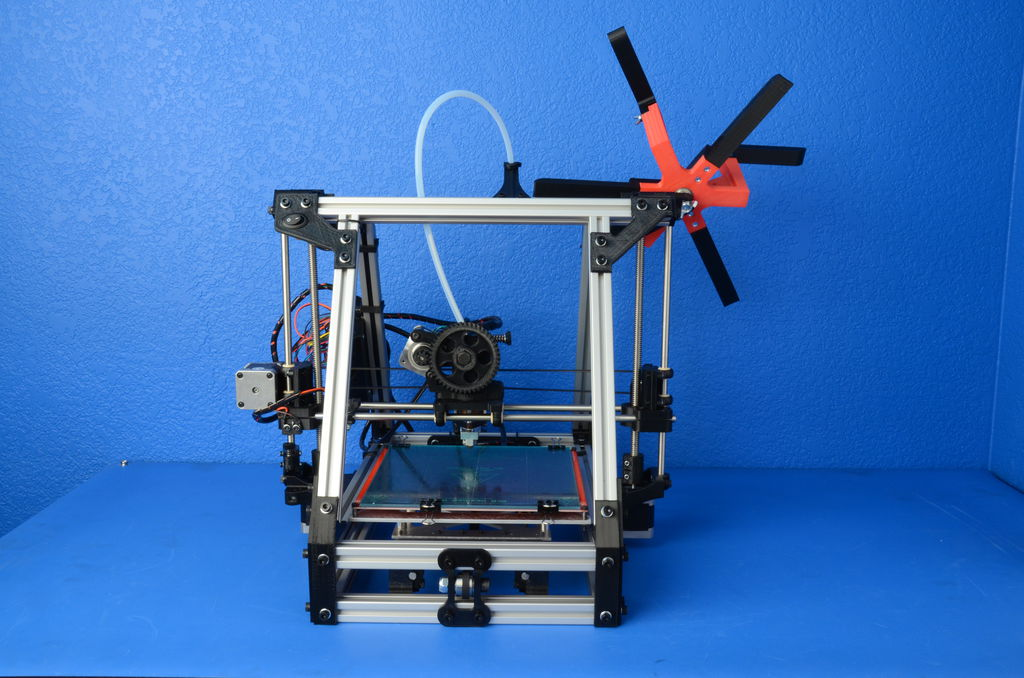
\includegraphics[keepaspectratio=true,height=0.40\textheight,width=1.00\textwidth,angle=0]{ao/ao-100-front.jpg}
 \caption{LulzBot AO-100 Front}
 \label{fig:ao-100-1-front}
\end{figure}

\begin{figure}[h!]
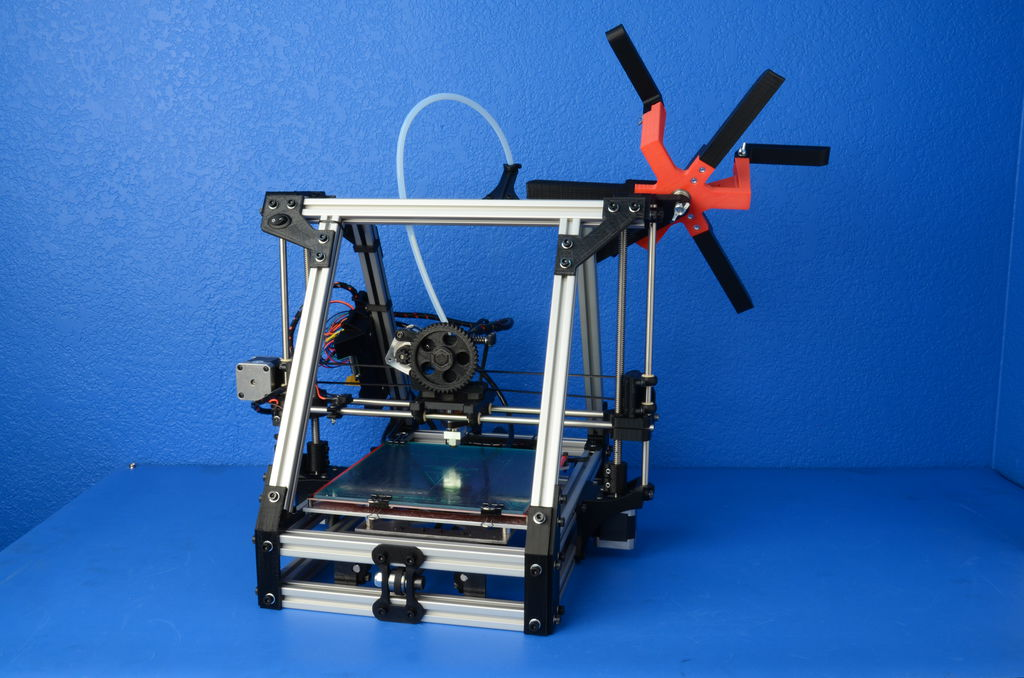
\includegraphics[keepaspectratio=true,height=0.40\textheight,width=1.00\textwidth,angle=0]{ao/ao-100-front-left.jpg}
 \caption{LulzBot AO-100 Front Left}
 \label{fig:ao-100-1-front-left}
\end{figure}

\begin{figure}[h!]
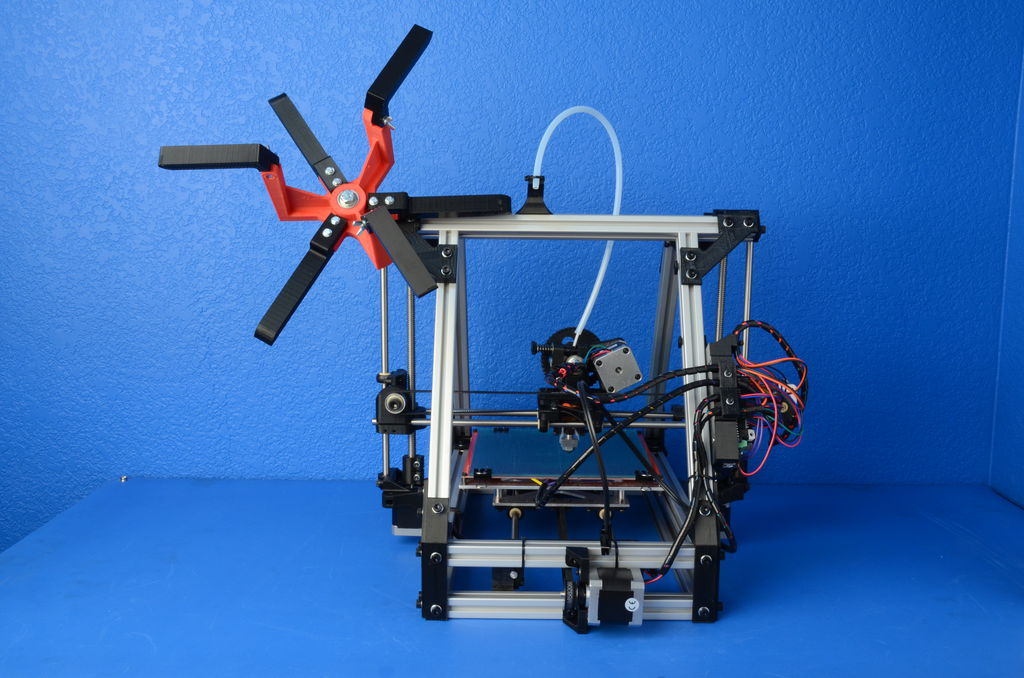
\includegraphics[keepaspectratio=true,height=0.40\textheight,width=1.00\textwidth,angle=0]{ao/ao-100-back.jpg}
 \caption{LulzBot AO-100 Back}
 \label{fig:ao-100-1-back}
\end{figure}

\begin{figure}[h!]
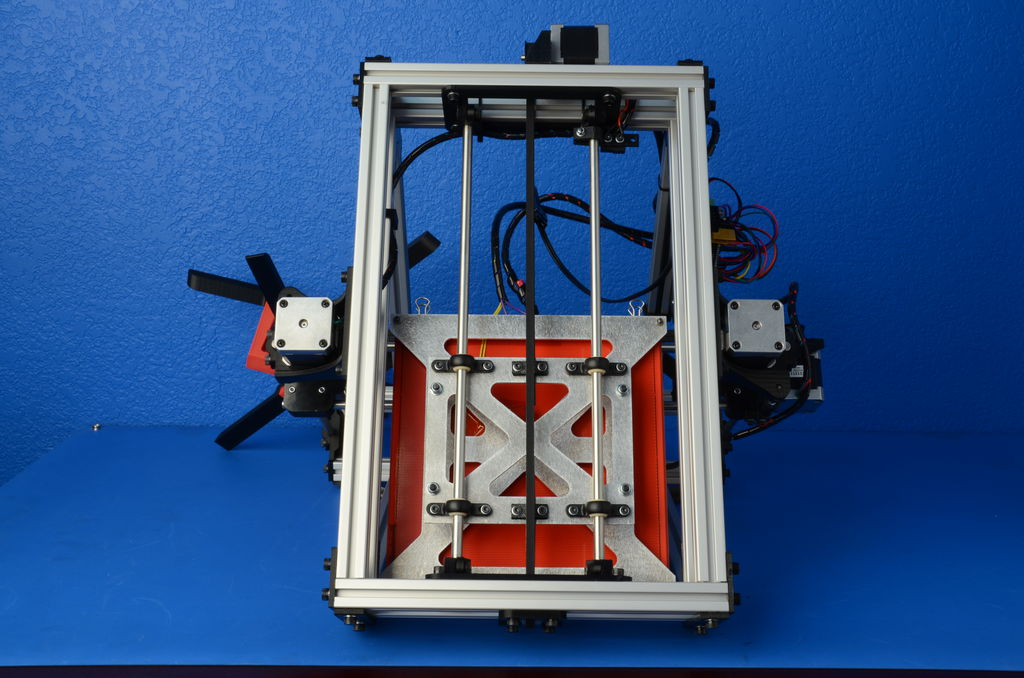
\includegraphics[keepaspectratio=true,height=0.40\textheight,width=1.00\textwidth,angle=0]{ao/ao-100-bottom.jpg}
 \caption{LulzBot AO-100 Bottom}
 \label{fig:ao-100-1-bottom}
\end{figure}

%\begin{figure}[h!]
%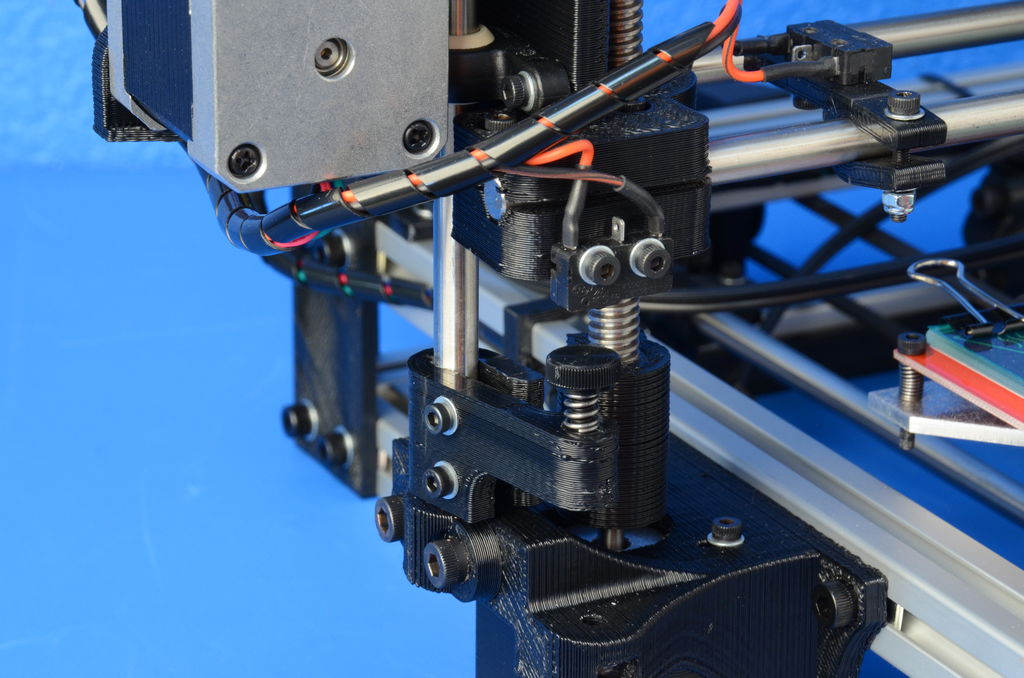
\includegraphics[keepaspectratio=true,height=0.40\textheight,width=1.00\textwidth,angle=0]{ao/ao-100-endstop.jpg}
% \caption{LulzBot AO-100 Endstop}
% \label{fig:ao-100-1-endstop}
%\end{figure}

\begin{figure}[h!]
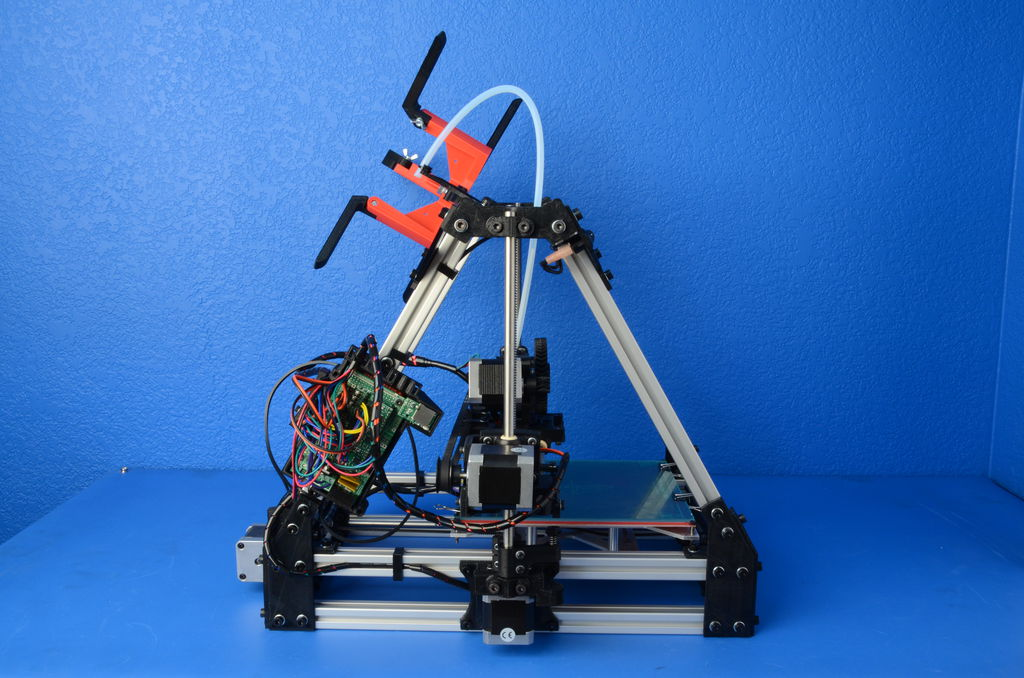
\includegraphics[keepaspectratio=true,height=0.40\textheight,width=1.00\textwidth,angle=0]{ao/ao-100-left.jpg}
 \caption{LulzBot AO-100 Front Left}
 \label{fig:ao-100-1-left}
\end{figure}

\begin{figure}[h!]
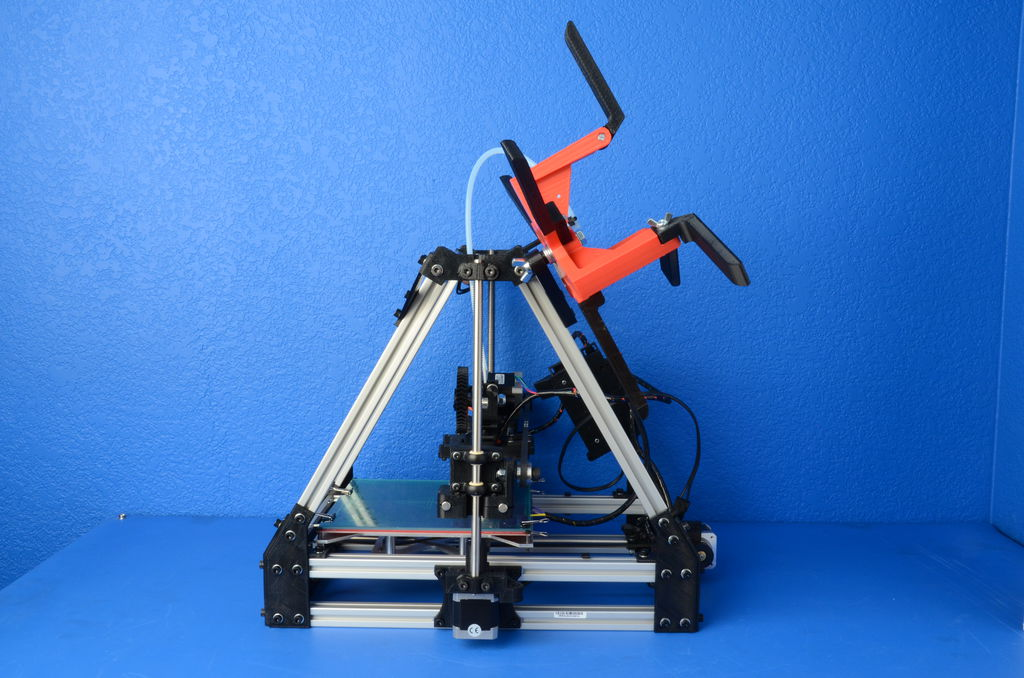
\includegraphics[keepaspectratio=true,height=0.40\textheight,width=1.00\textwidth,angle=0]{ao/ao-100-right.jpg}
 \caption{LulzBot AO-100 Front Right}
 \label{fig:ao-100-1-right}
\end{figure}

%\begin{figure}[h!]
%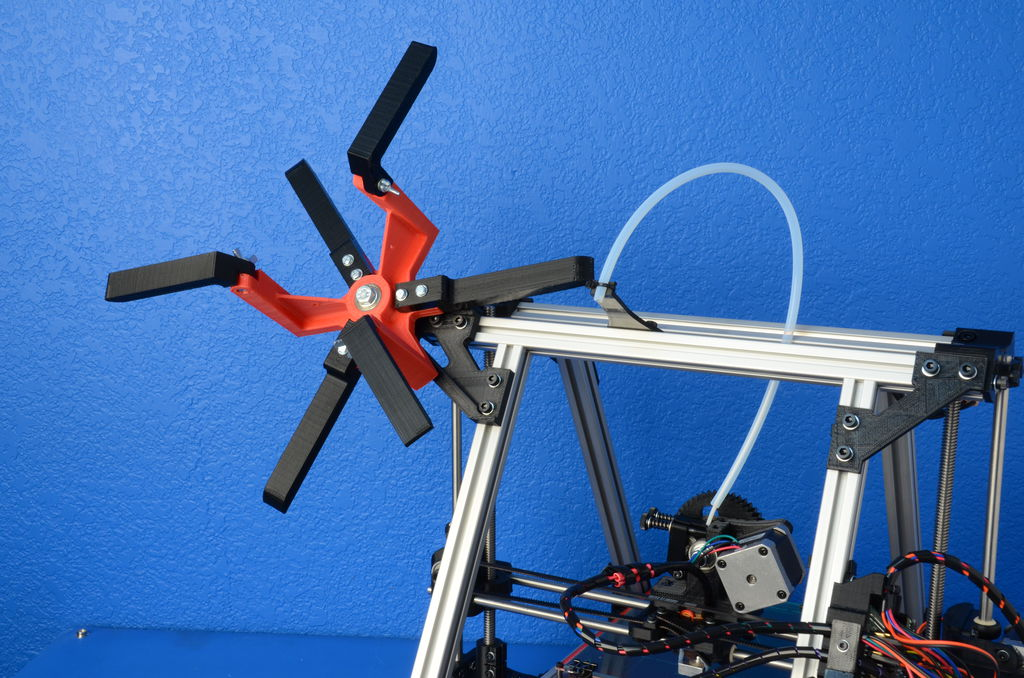
\includegraphics[keepaspectratio=true,height=0.40\textheight,width=1.00\textwidth,angle=0]{ao/ao-100-spool.jpg}
% \caption{LulzBot AO-100 Spool}
% \label{fig:ao-100-1-spool}
%\end{figure}

%\begin{figure}[h!]
%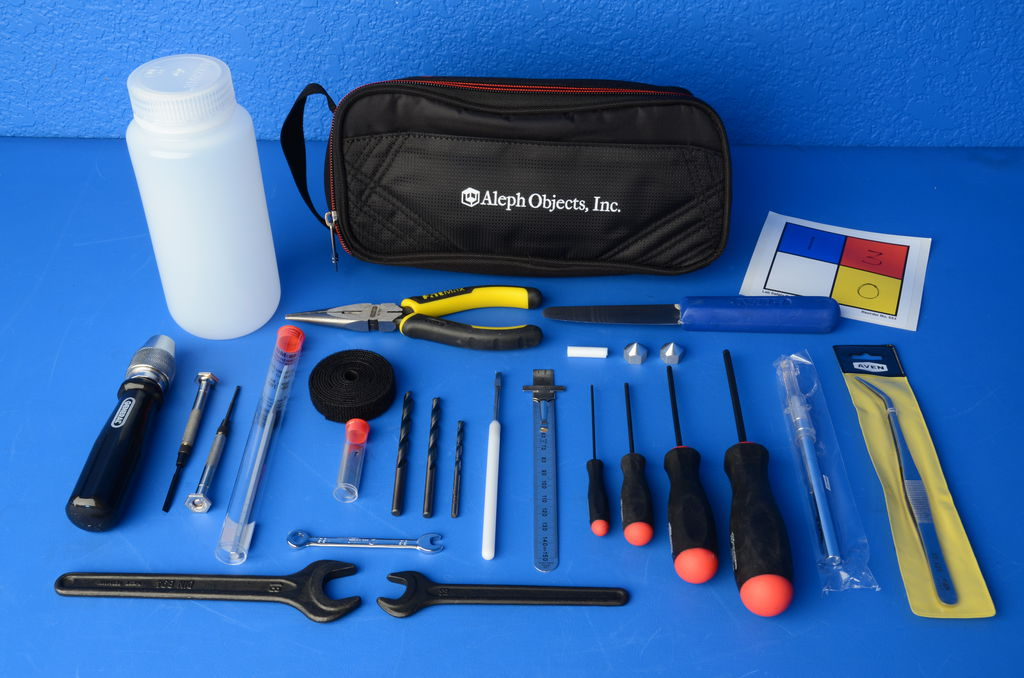
\includegraphics[keepaspectratio=true,height=0.40\textheight,width=1.00\textwidth,angle=0]{ao/ao-100-tools.jpg}
% \caption{LulzBot AO-100 Tools}
% \label{fig:ao-100-1-tools}
%\end{figure}

\begin{figure}[h!]
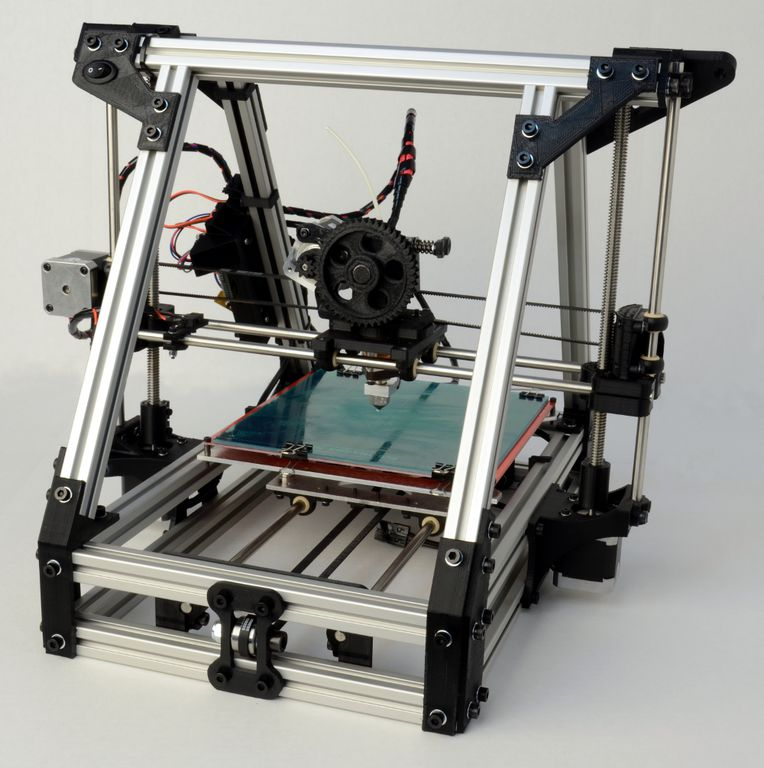
\includegraphics[keepaspectratio=true,height=0.40\textheight,width=1.00\textwidth,angle=0]{ao/ao-100-white.jpg}
 \caption{LulzBot AO-100}
 \label{fig:ao-100-1-white}
\end{figure}


%
% AO-101.tex
%
% History of LulzBot Printers
%
% Copyright (C) 2014, 2015 Aleph Objects, Inc.
%
% This document is licensed under the Creative Commons Attribution 4.0
% International Public License (CC BY-SA 4.0) by Aleph Objects, Inc.
%

\section{LulzBot AO-101}
LulzBot AO-101.

\begin{figure}[h!]
\thisfloatpagestyle{empty}
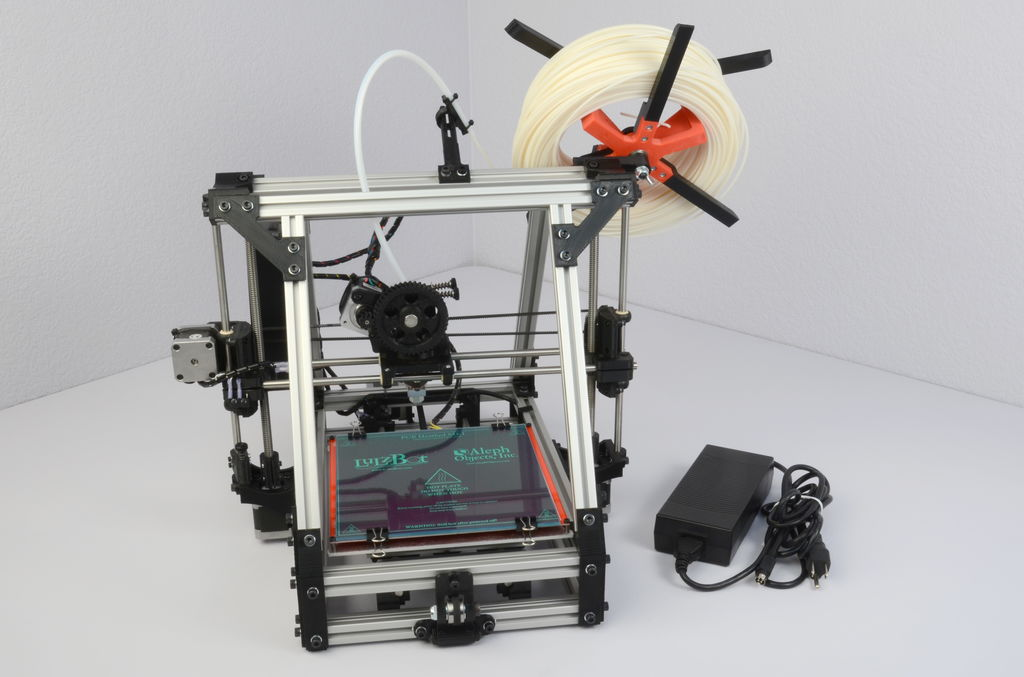
\includegraphics[keepaspectratio=true,height=0.40\textheight,width=1.00\textwidth,angle=0]{ao/ao-101.jpg}
 \caption{LulzBot AO-101}
 \label{fig:ao-101}
\end{figure}

\begin{figure}[h!]
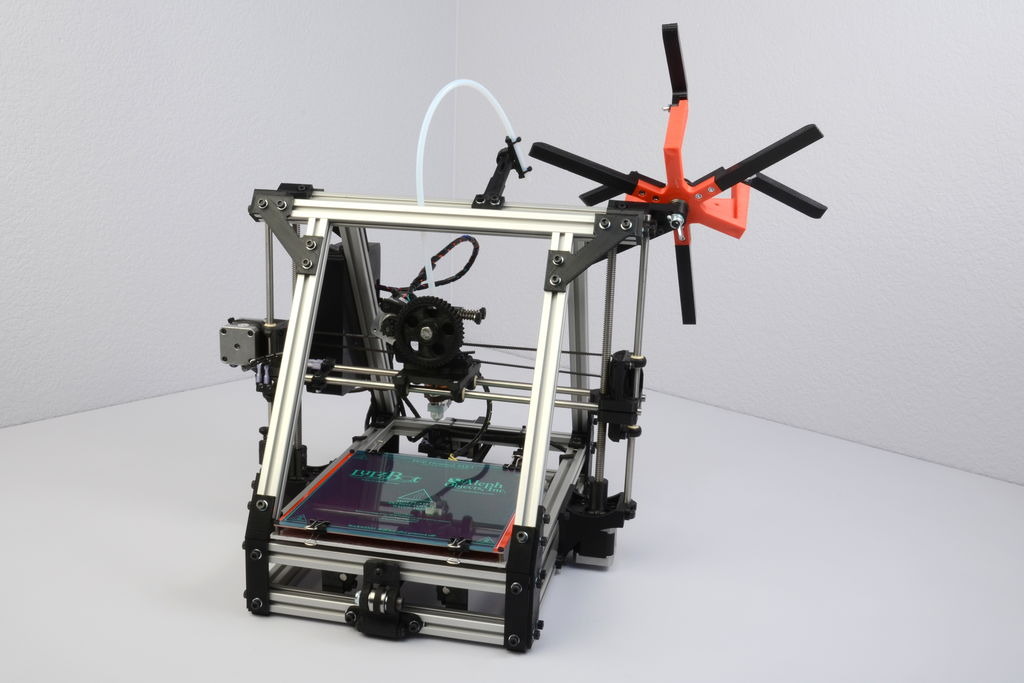
\includegraphics[keepaspectratio=true,height=0.40\textheight,width=1.00\textwidth,angle=0]{ao/ao-101-front.jpg}
 \caption{LulzBot AO-101 Front}
 \label{fig:ao-101-front}
\end{figure}

\begin{figure}[h!]
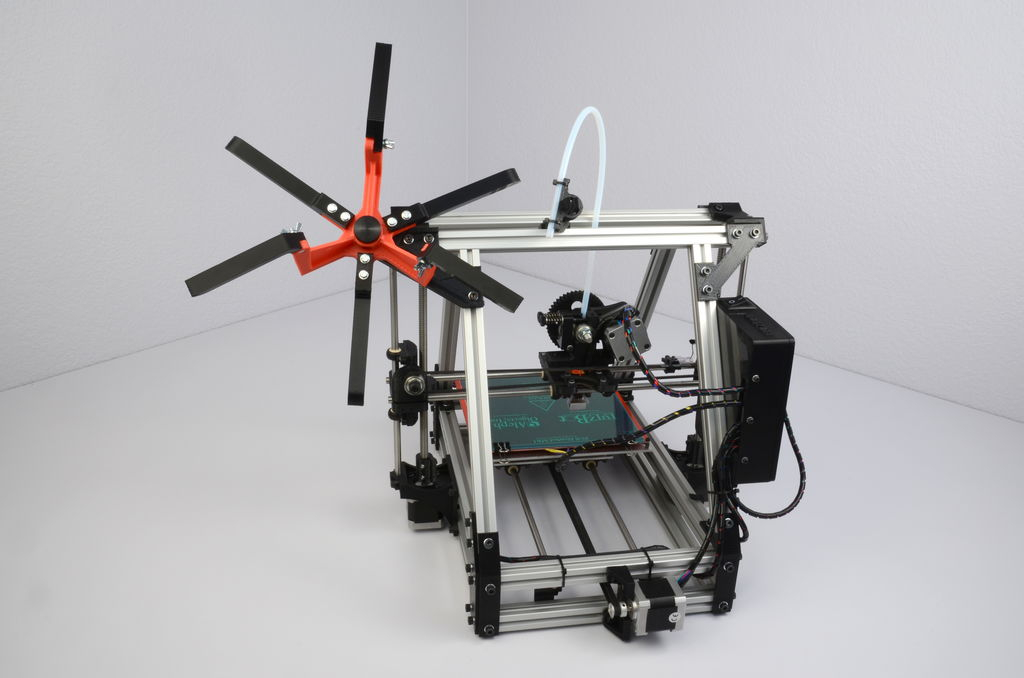
\includegraphics[keepaspectratio=true,height=0.40\textheight,width=1.00\textwidth,angle=0]{ao/ao-101-back.jpg}
 \caption{LulzBot AO-101 Back}
 \label{fig:ao-101-back}
\end{figure}

%\begin{figure}[h!]
%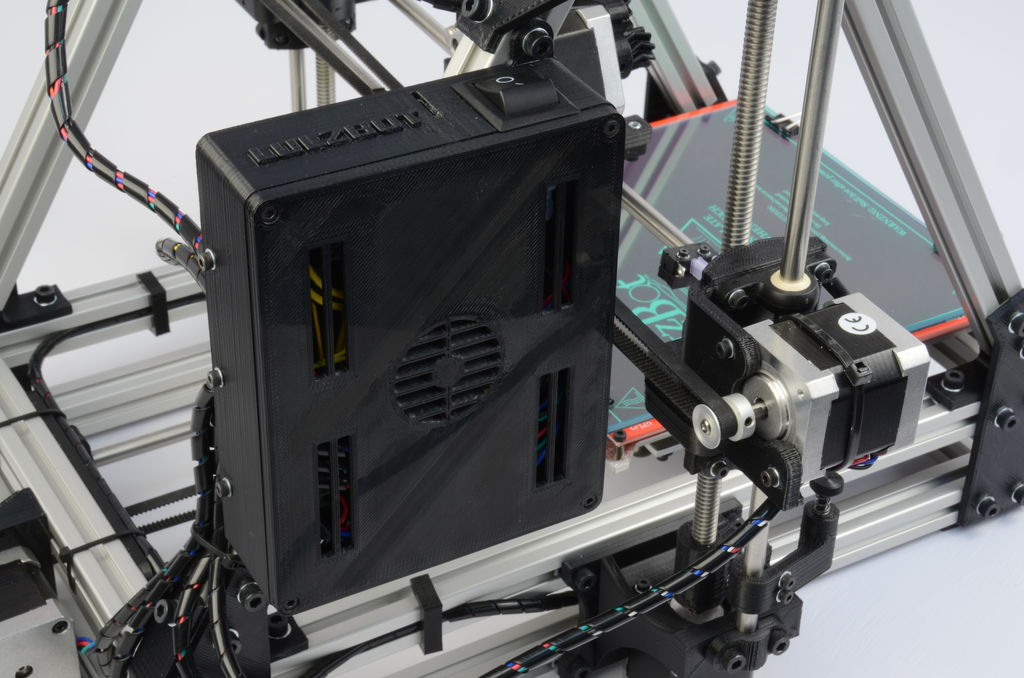
\includegraphics[keepaspectratio=true,height=0.40\textheight,width=1.00\textwidth,angle=0]{ao/ao-101-eleccase.jpg}
% \caption{LulzBot AO-101 Electronics Case}
% \label{fig:ao-101-eleccase}
%\end{figure}

%\begin{figure}[h!]
%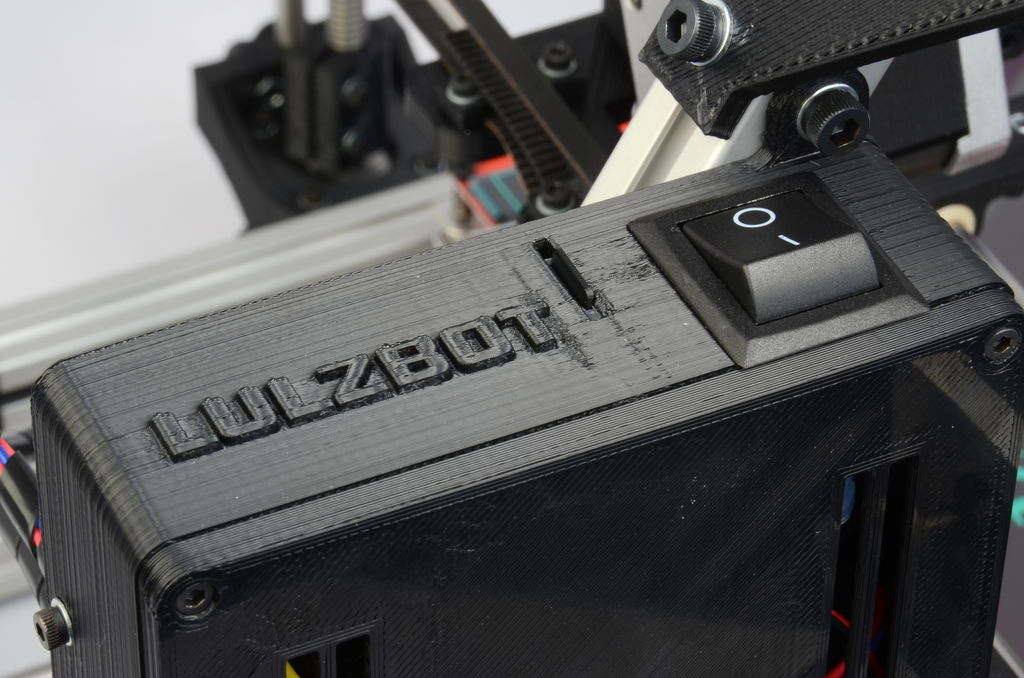
\includegraphics[keepaspectratio=true,height=0.40\textheight,width=1.00\textwidth,angle=0]{ao/ao-101-eleclulz.jpg}
% \caption{LulzBot AO-101 Electronics Case with LulzBot 3D Printed Text}
% \label{fig:ao-101-eleclulz}
%\end{figure}

%\begin{figure}[h!]
%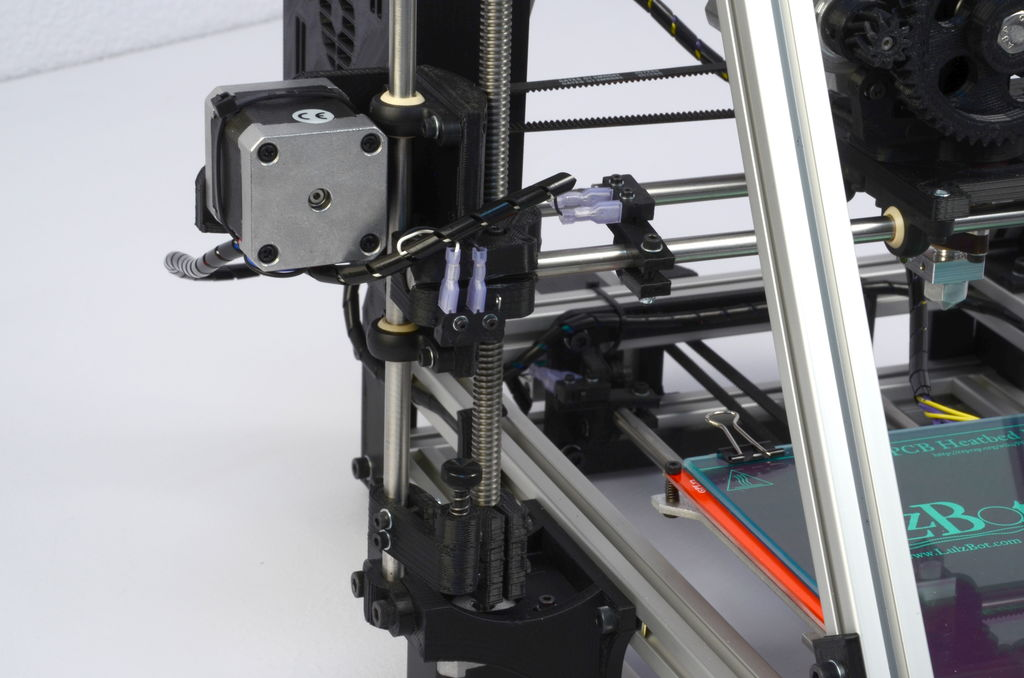
\includegraphics[keepaspectratio=true,height=0.40\textheight,width=1.00\textwidth,angle=0]{ao/ao-101-endstop.jpg}
% \caption{LulzBot AO-101 Endstop}
% \label{fig:ao-101-endstop}
%\end{figure}

\begin{figure}[h!]
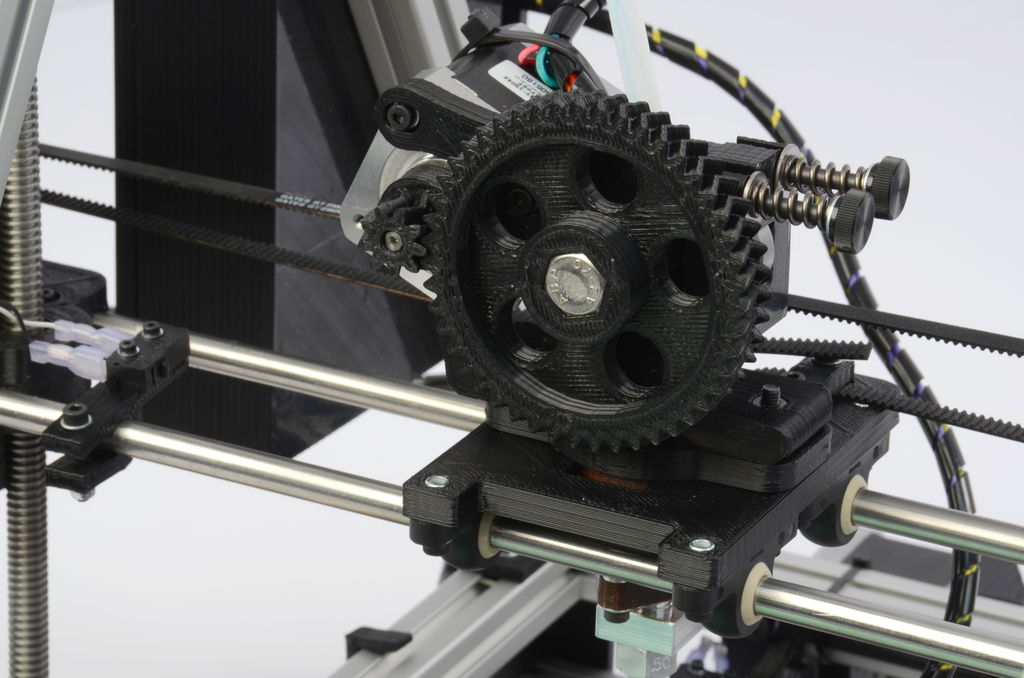
\includegraphics[keepaspectratio=true,height=0.40\textheight,width=1.00\textwidth,angle=0]{ao/ao-101-extruder.jpg}
 \caption{LulzBot AO-101 Extruder}
 \label{fig:ao-101-extruder}
\end{figure}

%\begin{figure}[h!]
%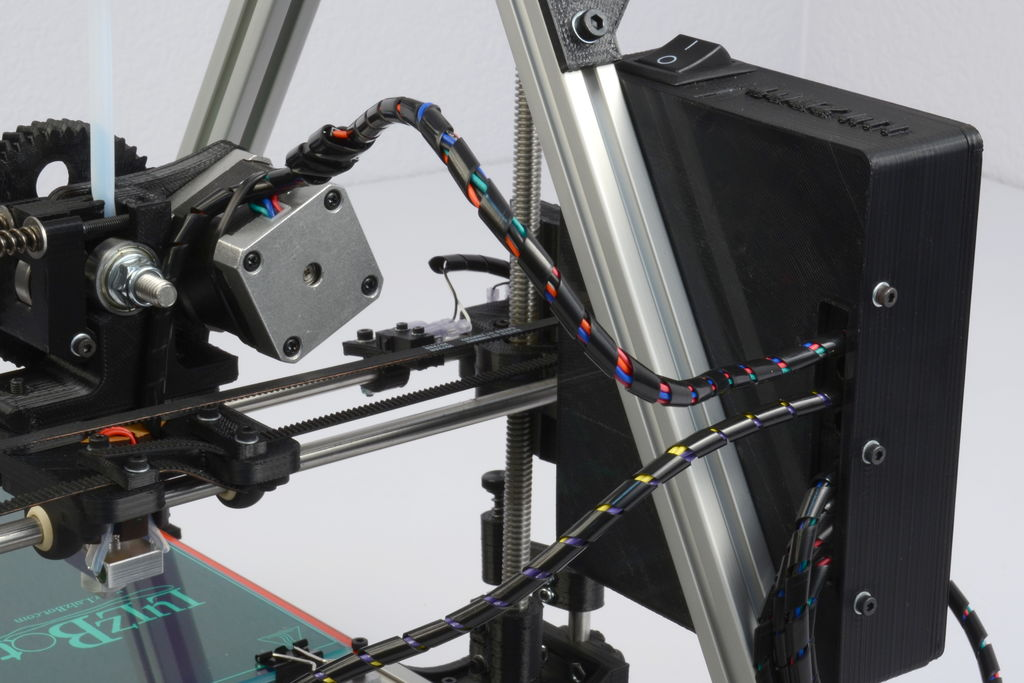
\includegraphics[keepaspectratio=true,height=0.40\textheight,width=1.00\textwidth,angle=0]{ao/ao-101-harness.jpg}
% \caption{LulzBot AO-101 Harness}
% \label{fig:ao-101-harness}
%\end{figure}

\begin{figure}[h!]
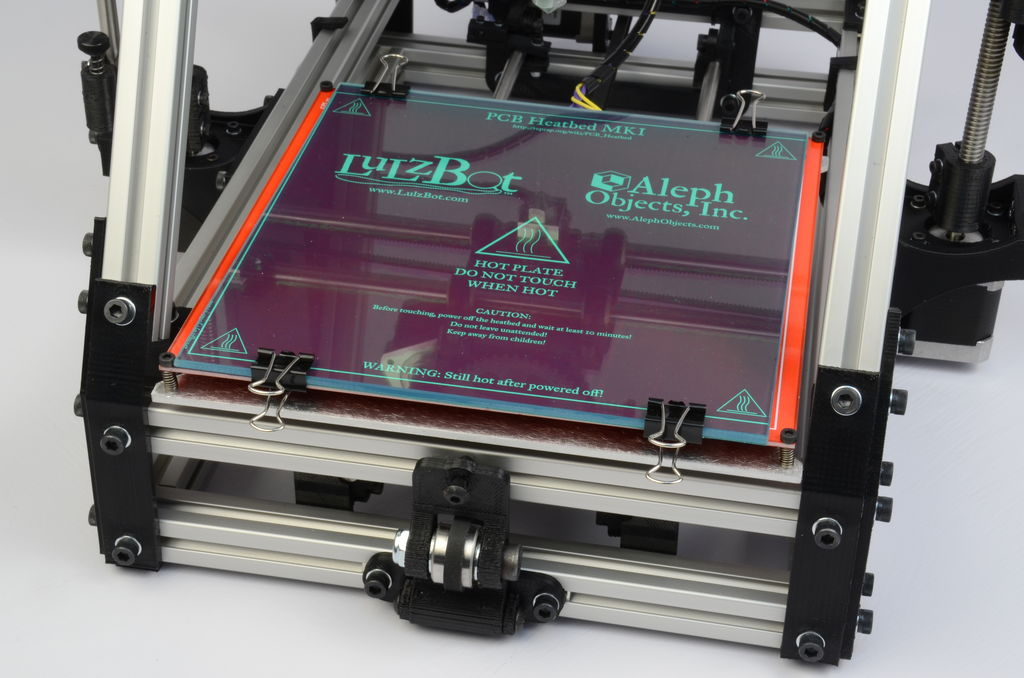
\includegraphics[keepaspectratio=true,height=0.40\textheight,width=1.00\textwidth,angle=0]{ao/ao-101-heatbed.jpg}
 \caption{LulzBot AO-101 Heatbed}
 \label{fig:ao-101-heatbed}
\end{figure}

%\begin{figure}[h!]
%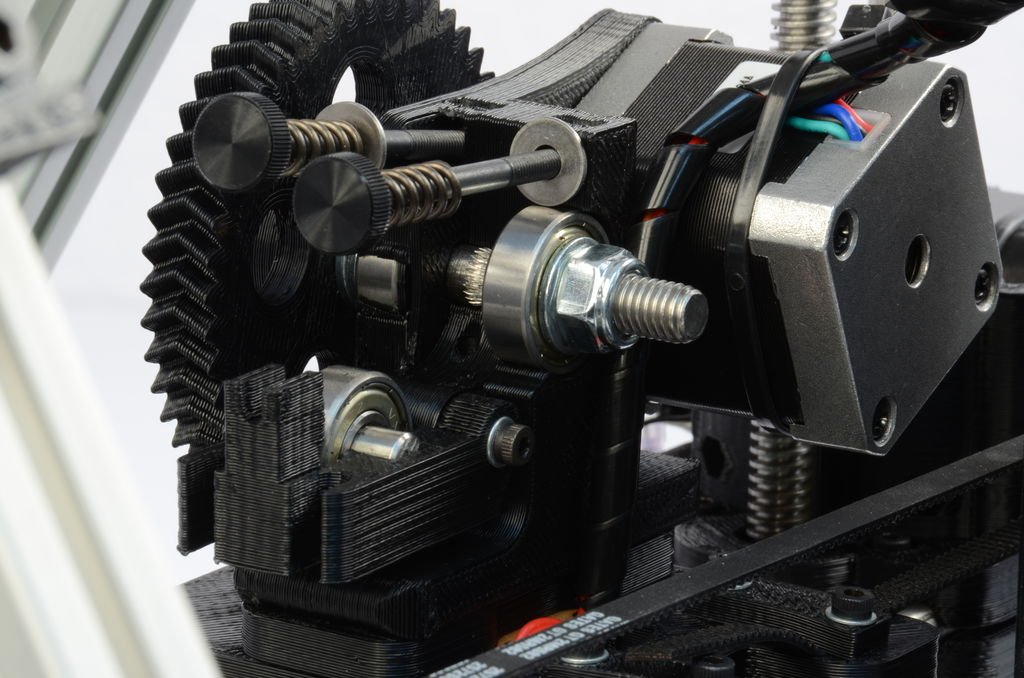
\includegraphics[keepaspectratio=true,height=0.40\textheight,width=1.00\textwidth,angle=0]{ao/ao-101-hobbed.jpg}
% \caption{LulzBot AO-101 Hobbed Bolt}
% \label{fig:ao-101-hobbed}
%\end{figure}

%\begin{figure}[h!]
%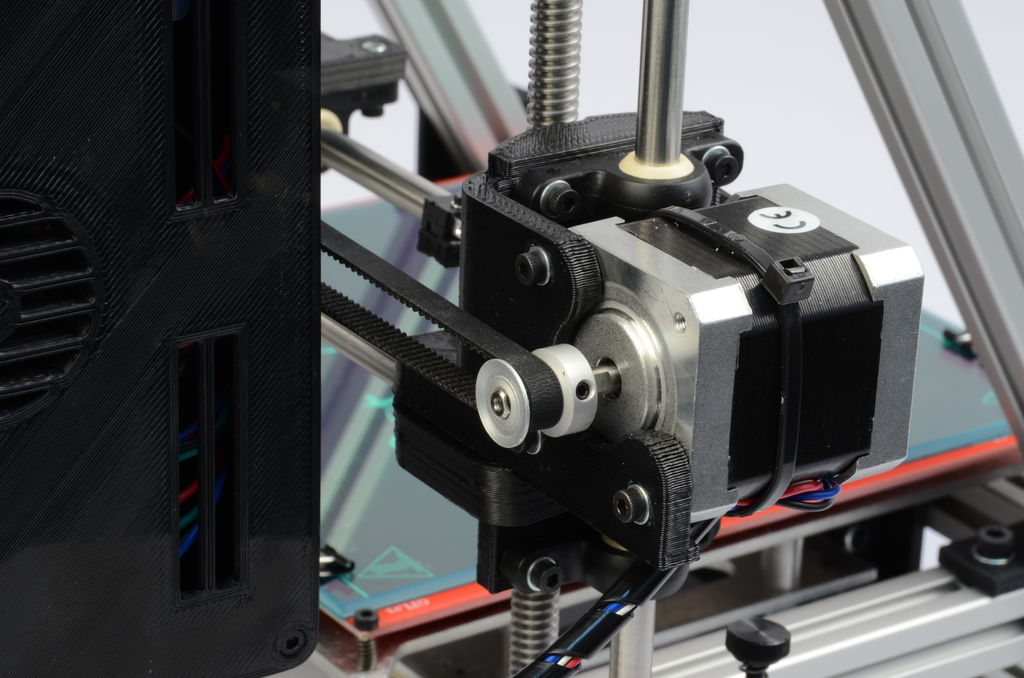
\includegraphics[keepaspectratio=true,height=0.40\textheight,width=1.00\textwidth,angle=0]{ao/ao-101-xmotor.jpg}
% \caption{LulzBot AO-101 X Motor}
% \label{fig:ao-101-xmotor}
%\end{figure}



